\documentclass{article}\usepackage[]{graphicx}\usepackage[]{color}
% maxwidth is the original width if it is less than linewidth
% otherwise use linewidth (to make sure the graphics do not exceed the margin)
\makeatletter
\def\maxwidth{ %
  \ifdim\Gin@nat@width>\linewidth
    \linewidth
  \else
    \Gin@nat@width
  \fi
}
\makeatother

\definecolor{fgcolor}{rgb}{0.345, 0.345, 0.345}
\newcommand{\hlnum}[1]{\textcolor[rgb]{0.686,0.059,0.569}{#1}}%
\newcommand{\hlstr}[1]{\textcolor[rgb]{0.192,0.494,0.8}{#1}}%
\newcommand{\hlcom}[1]{\textcolor[rgb]{0.678,0.584,0.686}{\textit{#1}}}%
\newcommand{\hlopt}[1]{\textcolor[rgb]{0,0,0}{#1}}%
\newcommand{\hlstd}[1]{\textcolor[rgb]{0.345,0.345,0.345}{#1}}%
\newcommand{\hlkwa}[1]{\textcolor[rgb]{0.161,0.373,0.58}{\textbf{#1}}}%
\newcommand{\hlkwb}[1]{\textcolor[rgb]{0.69,0.353,0.396}{#1}}%
\newcommand{\hlkwc}[1]{\textcolor[rgb]{0.333,0.667,0.333}{#1}}%
\newcommand{\hlkwd}[1]{\textcolor[rgb]{0.737,0.353,0.396}{\textbf{#1}}}%
\let\hlipl\hlkwb

\usepackage{framed}
\makeatletter
\newenvironment{kframe}{%
 \def\at@end@of@kframe{}%
 \ifinner\ifhmode%
  \def\at@end@of@kframe{\end{minipage}}%
  \begin{minipage}{\columnwidth}%
 \fi\fi%
 \def\FrameCommand##1{\hskip\@totalleftmargin \hskip-\fboxsep
 \colorbox{shadecolor}{##1}\hskip-\fboxsep
     % There is no \\@totalrightmargin, so:
     \hskip-\linewidth \hskip-\@totalleftmargin \hskip\columnwidth}%
 \MakeFramed {\advance\hsize-\width
   \@totalleftmargin\z@ \linewidth\hsize
   \@setminipage}}%
 {\par\unskip\endMakeFramed%
 \at@end@of@kframe}
\makeatother

\definecolor{shadecolor}{rgb}{.97, .97, .97}
\definecolor{messagecolor}{rgb}{0, 0, 0}
\definecolor{warningcolor}{rgb}{1, 0, 1}
\definecolor{errorcolor}{rgb}{1, 0, 0}
\newenvironment{knitrout}{}{} % an empty environment to be redefined in TeX

\usepackage{alltt}
\usepackage{amsmath} %This allows me to use the align functionality.
                     %If you find yourself trying to replicate
                     %something you found online, ensure you're
                     %loading the necessary packages!
\usepackage{amsfonts}%Math font
\usepackage{graphicx}%For including graphics
\usepackage{hyperref}%For Hyperlinks
\hypersetup{colorlinks = true,citecolor=black}
\usepackage{natbib}        %For the bibliography
\bibliographystyle{apalike}%For the bibliography
\usepackage[margin=1.0in]{geometry}
\usepackage{float}
\IfFileExists{upquote.sty}{\usepackage{upquote}}{}
\begin{document}
\noindent \textbf{MA 354: Data Analysis -- Fall 2021 -- Due 10/8 at 5p}\\%\\ gives you a new line
\noindent \textbf{Homework 2:}\vspace{1em}\\
\emph{Complete the following opportunities to use what we've talked about in class. These questions will be graded for correctness, communication and succinctness. Ensure you show your work and explain your logic in a legible and refined submission.}\\\vspace{1em}
%Comments -- anything after % is not put into the PDF

The starting jobs will be applied in alphabetical order (last name) for question two.
\begin{enumerate}
  \item \textbf{Solver:} provide a solution, if possible, and reasoning for the solution. \textbf{Due to group 10/5 or earlier.}
  \item \textbf{Code Checker:} provides a first check of the solver's worked solutions and ensures they are correct with a solid interpretation. 
  \item \textbf{Checker} checks the solution for completeness, proposes and implements changes if agreed upon by the group. Provides a short paragraph summarizing the discussion of proposals and their reason for acceptance or non-acceptance.
  \item \textbf{Double Checker} checks the solution for completeness, communication and polish. The Double Checker ensures that the solution is correct and highly polished for submission.
\end{enumerate}

\noindent For subsequent questions student roles will move down one position. The rolls change as follows.
\begin{enumerate}
  \item \textbf{Solver} $\Longrightarrow$ \textbf{Code Checker}
  \item \textbf{Code Checker} $\Longrightarrow$ \textbf{Checker}
  \item \textbf{Checker} $\Longrightarrow$ \textbf{Double Checker}
  \item \textbf{Double Checker} $\Longrightarrow$ \textbf{Solver}
\end{enumerate}
While students have assigned jobs for each question I encourage students to help 
each other complete the homework in collaboration.
\newpage
\begin{enumerate}
%%%%%%%%%%%%%%%%%%%%%%%%%%%%%%%%%%%%%%%%%%%%%%%%%%%%%%%%%%%%%%%%%%%%%%%%%%%%%%%%%%%%%%%%%%%
%%%%%%%%%%%%%%%%%%%%%%%%%%%%%%%%%%%%%%%%%%%%%%%%%%%%%%%%%%%%%%%%%%%%%%%%%%%%%%%%%%%%%%%%%%%
%%%%%%%%%  Question 4
%%%%%%%%%%%%%%%%%%%%%%%%%%%%%%%%%%%%%%%%%%%%%%%%%%%%%%%%%%%%%%%%%%%%%%%%%%%%%%%%%%%%%%%%%%%
%%%%%%%%%%%%%%%%%%%%%%%%%%%%%%%%%%%%%%%%%%%%%%%%%%%%%%%%%%%%%%%%%%%%%%%%%%%%%%%%%%%%%%%%%%%
\item Continue with the discrete distribution you selected for Question %\ref{Q3}.%
\begin{enumerate}
  %%%%%%%%%%%%%%%%%%%%%%%%%%%%%%%%%%%%%%%%%%%%%%%%%%%%%%%%%%%%%%%%%%%%%%%%%%%%%%%%%%%%%%%%%%%
  %%%%%%%%%  Part (a)
  %%%%%%%%%%%%%%%%%%%%%%%%%%%%%%%%%%%%%%%%%%%%%%%%%%%%%%%%%%%%%%%%%%%%%%%%%%%%%%%%%%%%%%%%%%%
  \item Provide the mean, standard deviation, skewness, and kurtosis of the PMF. 
  Ensure to interpret each.
\\
\\
Bernoulli Distribution:
\\



PMF:

\begin{align*}f\left(k;p\right) & =p^{k}\left(1-p\right)^{1-k} &  & \textrm{for \ensuremath{k\in\left\{ 0,1\right\} }}\end{align*}


Mean:

\[
E(X)=p
\]
\\
The mean represents the average or typical value that we would expect to see in a data set.\\
\\
Standard Deviation:

\[
\sigma=\sqrt{p\left(1-p\right)}
\]
\\
The standard deviation tells us how much the data in our data set varies from the mean. Data sets with lower standard deviations will have their data points grouped more tightly together, while data sets with higher standard deviations will have their data points more spread out.\\
\\
Skewness:

\[
\xi_{X}=\frac{\left(1-p\right)-p}{\sqrt{p\left(1-p\right)}}
\]
\\
The skewness tells us how symmetrical the data will be. If our data is positively or right-skewed, that means there will be a large grouping of data towards the left side of our distribution, with a long tail extending out to the right. Conversely, negatively or left-skewed data means there will be a large grouping of data towards the right side of our distribution, with a long tail extending out to the left. \\
\\
Kurtosis:

\[
\kappa_{Y}=3+\frac{1-6p\left(1-p\right)}{p\left(1-p\right)}
\]
\\
The kurtosis is used to tell us how thick or thin the peak and tails of our data distribution are. A data set with kurtosis greater than 3 will have a distribution that has thicker tails and a thinner peak. Conversely, a data set with kurtosis less than 3 will have thinner tails and a thicker peak.\\
\\
\\
\\
  %%%%%%%%%%%%%%%%%%%%%%%%%%%%%%%%%%%%%%%%%%%%%%%%%%%%%%%%%%%%%%%%%%%%%%%%%%%%%%%%%%%%%%%%%%%
  %%%%%%%%%  Part (b)
  %%%%%%%%%%%%%%%%%%%%%%%%%%%%%%%%%%%%%%%%%%%%%%%%%%%%%%%%%%%%%%%%%%%%%%%%%%%%%%%%%%%%%%%%%%%
  \item Generate a random sample of size $n=10, 25, 100$, and $1000$ for your 
  two sets of parameter(s). Calculate the sample mean, standard deviation, 
  skewness, and kurtosis. Interpret the results.
\begin{knitrout}
\definecolor{shadecolor}{rgb}{0.969, 0.969, 0.969}\color{fgcolor}\begin{kframe}
\begin{alltt}
\hlkwd{library}\hlstd{(e1071)}

\hlstd{even.10} \hlkwb{<-} \hlkwd{rbinom}\hlstd{(}\hlkwc{n}\hlstd{=}\hlnum{10}\hlstd{,}          \hlcom{#number of observations}
              \hlkwc{size}\hlstd{=}\hlnum{1}\hlstd{,}            \hlcom{#number of trials (size=1 for Bernoulli)}
              \hlkwc{prob}\hlstd{=}\hlnum{.5}\hlstd{)}           \hlcom{#probability of success}

\hlkwd{mean}\hlstd{(even.10)}                    \hlcom{#mean}
\end{alltt}
\begin{verbatim}
## [1] 0.7
\end{verbatim}
\begin{alltt}
\hlkwd{sd}\hlstd{(even.10)}                      \hlcom{#standard deviation}
\end{alltt}
\begin{verbatim}
## [1] 0.4830459
\end{verbatim}
\begin{alltt}
\hlkwd{skewness}\hlstd{(even.10)}                \hlcom{#skewness}
\end{alltt}
\begin{verbatim}
## [1] -0.7452708
\end{verbatim}
\begin{alltt}
\hlkwd{kurtosis}\hlstd{(even.10)}\hlopt{+}\hlnum{3}              \hlcom{#kurtosis}
\end{alltt}
\begin{verbatim}
## [1] 1.427143
\end{verbatim}
\begin{alltt}
\hlstd{even.25}  \hlkwb{<-} \hlkwd{rbinom}\hlstd{(}\hlkwc{n}\hlstd{=}\hlnum{25}\hlstd{,}         \hlcom{#number of observations}
              \hlkwc{size}\hlstd{=}\hlnum{1}\hlstd{,}            \hlcom{#number of trials (size=1 for Bernoulli)}
              \hlkwc{prob}\hlstd{=}\hlnum{.5}\hlstd{)}           \hlcom{#probability of success}

\hlkwd{mean}\hlstd{(even.25)}                    \hlcom{#mean}
\end{alltt}
\begin{verbatim}
## [1] 0.48
\end{verbatim}
\begin{alltt}
\hlkwd{sd}\hlstd{(even.25)}                      \hlcom{#standard deviation}
\end{alltt}
\begin{verbatim}
## [1] 0.509902
\end{verbatim}
\begin{alltt}
\hlkwd{skewness}\hlstd{(even.25)}                \hlcom{#skewness}
\end{alltt}
\begin{verbatim}
## [1] 0.0753086
\end{verbatim}
\begin{alltt}
\hlkwd{kurtosis}\hlstd{(even.25)}\hlopt{+}\hlnum{3}              \hlcom{#kurtosis}
\end{alltt}
\begin{verbatim}
## [1] 0.9275077
\end{verbatim}
\begin{alltt}
\hlstd{even.100} \hlkwb{<-} \hlkwd{rbinom}\hlstd{(}\hlkwc{n}\hlstd{=}\hlnum{100}\hlstd{,}        \hlcom{#number of observations}
              \hlkwc{size}\hlstd{=}\hlnum{1}\hlstd{,}            \hlcom{#number of trials (size=1 for Bernoulli)}
              \hlkwc{prob}\hlstd{=}\hlnum{.5}\hlstd{)}           \hlcom{#probability of success}

\hlkwd{mean}\hlstd{(even.100)}                   \hlcom{#mean}
\end{alltt}
\begin{verbatim}
## [1] 0.52
\end{verbatim}
\begin{alltt}
\hlkwd{sd}\hlstd{(even.100)}                     \hlcom{#standard deviation}
\end{alltt}
\begin{verbatim}
## [1] 0.5021167
\end{verbatim}
\begin{alltt}
\hlkwd{skewness}\hlstd{(even.100)}               \hlcom{#skewness}
\end{alltt}
\begin{verbatim}
## [1] -0.07886612
\end{verbatim}
\begin{alltt}
\hlkwd{kurtosis}\hlstd{(even.100)}\hlopt{+}\hlnum{3}             \hlcom{#kurtosis}
\end{alltt}
\begin{verbatim}
## [1] 0.9863827
\end{verbatim}
\begin{alltt}
\hlstd{even.1000} \hlkwb{<-} \hlkwd{rbinom}\hlstd{(}\hlkwc{n}\hlstd{=}\hlnum{1000}\hlstd{,}      \hlcom{#number of observations}
              \hlkwc{size}\hlstd{=}\hlnum{1}\hlstd{,}            \hlcom{#number of trials (size=1 for Bernoulli)}
              \hlkwc{prob}\hlstd{=}\hlnum{.5}\hlstd{)}           \hlcom{#probability of success}

\hlkwd{mean}\hlstd{(even.1000)}                  \hlcom{#mean}
\end{alltt}
\begin{verbatim}
## [1] 0.455
\end{verbatim}
\begin{alltt}
\hlkwd{sd}\hlstd{(even.1000)}                    \hlcom{#standard deviation}
\end{alltt}
\begin{verbatim}
## [1] 0.4982201
\end{verbatim}
\begin{alltt}
\hlkwd{skewness}\hlstd{(even.1000)}              \hlcom{#skewness}
\end{alltt}
\begin{verbatim}
## [1] 0.1804624
\end{verbatim}
\begin{alltt}
\hlkwd{kurtosis}\hlstd{(even.1000)}\hlopt{+}\hlnum{3}            \hlcom{#kurtosis}
\end{alltt}
\begin{verbatim}
## [1] 1.0306
\end{verbatim}
\begin{alltt}
\hlstd{uneven.10} \hlkwb{<-} \hlkwd{rbinom}\hlstd{(}\hlkwc{n}\hlstd{=}\hlnum{10}\hlstd{,}        \hlcom{#number of observations}
                  \hlkwc{size}\hlstd{=}\hlnum{1}\hlstd{,}        \hlcom{#number of trials (size=1 for Bernoulli)}
                  \hlkwc{prob}\hlstd{=}\hlnum{.7}\hlstd{)}       \hlcom{#probability of success}

\hlkwd{mean}\hlstd{(uneven.10)}                  \hlcom{#mean}
\end{alltt}
\begin{verbatim}
## [1] 0.7
\end{verbatim}
\begin{alltt}
\hlkwd{sd}\hlstd{(uneven.10)}                    \hlcom{#standard deviation}
\end{alltt}
\begin{verbatim}
## [1] 0.4830459
\end{verbatim}
\begin{alltt}
\hlkwd{skewness}\hlstd{(uneven.10)}              \hlcom{#skewness}
\end{alltt}
\begin{verbatim}
## [1] -0.7452708
\end{verbatim}
\begin{alltt}
\hlkwd{kurtosis}\hlstd{(uneven.10)}\hlopt{+}\hlnum{3}            \hlcom{#kurtosis}
\end{alltt}
\begin{verbatim}
## [1] 1.427143
\end{verbatim}
\begin{alltt}
\hlstd{uneven.25}  \hlkwb{<-} \hlkwd{rbinom}\hlstd{(}\hlkwc{n}\hlstd{=}\hlnum{25}\hlstd{,}       \hlcom{#number of observations}
                   \hlkwc{size}\hlstd{=}\hlnum{1}\hlstd{,}       \hlcom{#number of trials (size=1 for Bernoulli)}
                   \hlkwc{prob}\hlstd{=}\hlnum{.7}\hlstd{)}      \hlcom{#probability of success}

\hlkwd{mean}\hlstd{(uneven.25)}                  \hlcom{#mean}
\end{alltt}
\begin{verbatim}
## [1] 0.8
\end{verbatim}
\begin{alltt}
\hlkwd{sd}\hlstd{(uneven.25)}                    \hlcom{#standard deviation}
\end{alltt}
\begin{verbatim}
## [1] 0.4082483
\end{verbatim}
\begin{alltt}
\hlkwd{skewness}\hlstd{(uneven.25)}              \hlcom{#skewness}
\end{alltt}
\begin{verbatim}
## [1] -1.410906
\end{verbatim}
\begin{alltt}
\hlkwd{kurtosis}\hlstd{(uneven.25)}\hlopt{+}\hlnum{3}            \hlcom{#kurtosis}
\end{alltt}
\begin{verbatim}
## [1] 2.9952
\end{verbatim}
\begin{alltt}
\hlstd{uneven.100} \hlkwb{<-} \hlkwd{rbinom}\hlstd{(}\hlkwc{n}\hlstd{=}\hlnum{100}\hlstd{,}      \hlcom{#number of observations}
                   \hlkwc{size}\hlstd{=}\hlnum{1}\hlstd{,}       \hlcom{#number of trials (size=1 for Bernoulli)}
                   \hlkwc{prob}\hlstd{=}\hlnum{.7}\hlstd{)}      \hlcom{#probability of success}

\hlkwd{mean}\hlstd{(uneven.100)}                 \hlcom{#mean}
\end{alltt}
\begin{verbatim}
## [1] 0.71
\end{verbatim}
\begin{alltt}
\hlkwd{sd}\hlstd{(uneven.100)}                   \hlcom{#standard deviation}
\end{alltt}
\begin{verbatim}
## [1] 0.456048
\end{verbatim}
\begin{alltt}
\hlkwd{skewness}\hlstd{(uneven.100)}             \hlcom{#skewness}
\end{alltt}
\begin{verbatim}
## [1] -0.9117461
\end{verbatim}
\begin{alltt}
\hlkwd{kurtosis}\hlstd{(uneven.100)}\hlopt{+}\hlnum{3}           \hlcom{#kurtosis}
\end{alltt}
\begin{verbatim}
## [1] 1.819778
\end{verbatim}
\begin{alltt}
\hlstd{uneven.1000} \hlkwb{<-} \hlkwd{rbinom}\hlstd{(}\hlkwc{n}\hlstd{=}\hlnum{1000}\hlstd{,}    \hlcom{#number of observations}
                    \hlkwc{size}\hlstd{=}\hlnum{1}\hlstd{,}      \hlcom{#number of trials (size=1 for Bernoulli)}
                    \hlkwc{prob}\hlstd{=}\hlnum{.7}\hlstd{)}     \hlcom{#probability of success}

\hlkwd{mean}\hlstd{(uneven.1000)}                \hlcom{#mean}
\end{alltt}
\begin{verbatim}
## [1] 0.712
\end{verbatim}
\begin{alltt}
\hlkwd{sd}\hlstd{(uneven.1000)}                  \hlcom{#standard deviation}
\end{alltt}
\begin{verbatim}
## [1] 0.4530577
\end{verbatim}
\begin{alltt}
\hlkwd{skewness}\hlstd{(uneven.1000)}            \hlcom{#skewness}
\end{alltt}
\begin{verbatim}
## [1] -0.9349273
\end{verbatim}
\begin{alltt}
\hlkwd{kurtosis}\hlstd{(uneven.1000)}\hlopt{+}\hlnum{3}          \hlcom{#kurtosis}
\end{alltt}
\begin{verbatim}
## [1] 1.872965
\end{verbatim}
\end{kframe}
\end{knitrout}
Calculated Mean, Standard Deviation, Skewness and Kurtosis:

\[
\]

For $p=.5$:

\[
\]

Mean:

\[
E(X)=.5
\]

Standard Deviation:

\begin{align*}\sigma & =\sqrt{.5\left(1-.5\right)}\\
\\
 & =.5
\end{align*}

Skewness:

\begin{align*}\xi_{X} & =\frac{\left(1-.5\right)-.5}{\sqrt{.5\left(1-.5\right)}}\\
\\
 & =0
\end{align*}

Kurtosis:

\begin{align*}\kappa_{Y} & =3+\frac{1-6\left(.5\right)\left(1-.5\right)}{.5\left(1-.5\right)}\\
\\
 & =1
\end{align*}

\[
\]

For $p=.7$:

\[
\]

Mean:

\[
E(X)=.7
\]

Standard Deviation:

\begin{align*}\sigma & =\sqrt{.7\left(1-.7\right)}\\
\\
 & \approx.45825
\end{align*}

Skewness:

\begin{align*}\xi_{X} & =\frac{\left(1-.7\right)-.7}{\sqrt{.7\left(1-.7\right)}}\\
\\
 & \approx-.87287
\end{align*}

Kurtosis:

\begin{align*}\kappa_{Y} & =3+\frac{1-6\left(.7\right)\left(1-.7\right)}{.7\left(1-.7\right)}\\
\\
 & \approx1.76190
\end{align*}\\
By comparing the values we received computationally to the values that we calculated we can see that as our random sample size $n$ increases, the computational values that we received for our mean, standard deviation, skewness, and kurtosis tended to approach the actual values for the distribution that we calculated.\\
\\
  %%%%%%%%%%%%%%%%%%%%%%%%%%%%%%%%%%%%%%%%%%%%%%%%%%%%%%%%%%%%%%%%%%%%%%%%%%%%%%%%%%%%%%%%%%%
  %%%%%%%%%  Part (c)
  %%%%%%%%%%%%%%%%%%%%%%%%%%%%%%%%%%%%%%%%%%%%%%%%%%%%%%%%%%%%%%%%%%%%%%%%%%%%%%%%%%%%%%%%%%%
  \item Generate a random sample of size $n=10$ for your two sets of parameter(s).
  Calculate the method of moments estimator(s) and maximum likelihood estimator(s).
  In a $1 \times 2$ grid, plot a histogram (with bin size 1) of each set of data 
  with (1) the method of moments estimated distribution, (2) the maximum likelihood 
  estimated distribution, and superimpose the true distribution in both.
\begin{knitrout}
\definecolor{shadecolor}{rgb}{0.969, 0.969, 0.969}\color{fgcolor}\begin{kframe}
\begin{alltt}
\hlkwd{library}\hlstd{(tidyverse)}
\hlkwd{library}\hlstd{(patchwork)}

\hlstd{second.moment} \hlkwb{<-} \hlkwa{function}\hlstd{(}\hlkwc{data}\hlstd{,} \hlkwc{x.bar}\hlstd{)\{}  \hlcom{#function to find the second moment}
  \hlstd{temp} \hlkwb{=} \hlnum{0}
  \hlkwa{for}\hlstd{(i} \hlkwa{in} \hlstd{data)\{}
    \hlstd{temp} \hlkwb{=} \hlstd{temp} \hlopt{+} \hlstd{(i} \hlopt{-} \hlstd{x.bar)}\hlopt{^}\hlnum{2}
  \hlstd{\}}
  \hlkwd{return} \hlstd{(temp}\hlopt{/}\hlkwd{length}\hlstd{(data))}
\hlstd{\}}

\hlstd{MOM.bernoulli} \hlkwb{<-} \hlkwa{function}\hlstd{(}\hlkwc{data}\hlstd{)\{}          \hlcom{#function to find the MOM Estimator for p in a Bernoulli distribution}
  \hlstd{mu.hat} \hlkwb{<-} \hlkwd{mean}\hlstd{(data)}
  \hlstd{var.hat} \hlkwb{<-} \hlkwd{second.moment}\hlstd{(data,mu.hat)}
  \hlstd{p.hat} \hlkwb{<-} \hlstd{(mu.hat}\hlopt{-}\hlstd{var.hat)}\hlopt{/}\hlstd{mu.hat}
  \hlkwd{return}\hlstd{(p.hat)}
\hlstd{\}}

\hlcom{# Negative of the Likelihood function}
\hlstd{bernoulliLogLik.neg} \hlkwb{<-} \hlkwa{function}\hlstd{(}\hlkwc{par}\hlstd{,} \hlkwc{data}\hlstd{)\{}
  \hlopt{-}\hlkwd{sum}\hlstd{(}\hlkwd{dbinom}\hlstd{(}\hlkwc{x}\hlstd{=data,} \hlkwc{prob}\hlstd{=par,} \hlkwc{size}\hlstd{=}\hlnum{1}\hlstd{,} \hlkwc{log}\hlstd{=}\hlnum{TRUE}\hlstd{))\}} \hlcom{#Sum is negative, as we are looking for a min with optim}

\hlstd{MLE.bernoulli} \hlkwb{<-} \hlkwa{function}\hlstd{(}\hlkwc{data}\hlstd{)\{}
  \hlstd{MLE} \hlkwb{<-} \hlkwd{optim}\hlstd{(}\hlkwc{par} \hlstd{=} \hlnum{.5}\hlstd{,}               \hlcom{# best guess for the parameter}
               \hlkwc{fn} \hlstd{= bernoulliLogLik.neg,}   \hlcom{# function to minimize}
               \hlkwc{data} \hlstd{= data,}       \hlcom{# data (an argument to fn)}
               \hlkwc{method} \hlstd{=} \hlstr{"Brent"}\hlstd{,}       \hlcom{# required for univariate optimization}
               \hlkwc{lower} \hlstd{=} \hlnum{0}\hlstd{,}              \hlcom{# lowest possible lambda}
               \hlkwc{upper} \hlstd{=} \hlnum{1}\hlstd{)}              \hlcom{# reasonable upper bound}

  \hlcom{# Note that our mle is hat(lambda) = xbar }
  \hlkwd{return}\hlstd{(MLE}\hlopt{$}\hlstd{par)}
\hlstd{\}}

\hlstd{bernoulli.plot} \hlkwb{<-} \hlkwa{function}\hlstd{(}\hlkwc{data}\hlstd{)\{}

  \hlstd{dfActual} \hlkwb{<-} \hlkwd{data.frame}\hlstd{(}\hlkwd{matrix}\hlstd{(}\hlkwc{nrow} \hlstd{=} \hlnum{2}\hlstd{,} \hlkwc{ncol} \hlstd{=} \hlnum{2}\hlstd{))}
  \hlkwd{colnames}\hlstd{(dfActual)} \hlkwb{<-} \hlkwd{c}\hlstd{(}\hlstr{"Prop"}\hlstd{,}\hlstr{"Value"}\hlstd{)}
  \hlkwd{rownames}\hlstd{(dfActual)} \hlkwb{<-} \hlkwd{c}\hlstd{(}\hlstr{"0"}\hlstd{,}\hlstr{"1"}\hlstd{)}

  \hlstd{ActualTab} \hlkwb{<-} \hlkwd{as.data.frame}\hlstd{(data)} \hlopt \hlkwd{group_by}\hlstd{(data)} \hlopt
    \hlkwd{summarize}\hlstd{(}\hlkwc{count} \hlstd{=} \hlkwd{n}\hlstd{())} \hlcom{# Calculate the counts}

  \hlstd{dfActual[}\hlnum{1}\hlstd{,}\hlnum{1}\hlstd{]} \hlkwb{<-} \hlkwd{prop.table}\hlstd{(ActualTab}\hlopt{$}\hlstd{count)[}\hlnum{1}\hlstd{]}
  \hlstd{dfActual[}\hlnum{2}\hlstd{,}\hlnum{1}\hlstd{]} \hlkwb{<-} \hlkwd{prop.table}\hlstd{(ActualTab}\hlopt{$}\hlstd{count)[}\hlnum{2}\hlstd{]}
  \hlstd{dfActual[}\hlnum{1}\hlstd{,}\hlnum{2}\hlstd{]} \hlkwb{<-} \hlnum{0}
  \hlstd{dfActual[}\hlnum{2}\hlstd{,}\hlnum{2}\hlstd{]} \hlkwb{<-} \hlnum{1}


  \hlstd{dfEstimate} \hlkwb{<-} \hlkwd{data.frame}\hlstd{(}\hlkwd{matrix}\hlstd{(}\hlkwc{nrow} \hlstd{=} \hlnum{2}\hlstd{,} \hlkwc{ncol} \hlstd{=} \hlnum{2}\hlstd{))}
  \hlkwd{colnames}\hlstd{(dfEstimate)} \hlkwb{<-} \hlkwd{c}\hlstd{(}\hlstr{"Prop"}\hlstd{,}\hlstr{"Value"}\hlstd{)}
  \hlkwd{rownames}\hlstd{(dfEstimate)} \hlkwb{<-} \hlkwd{c}\hlstd{(}\hlstr{"0"}\hlstd{,}\hlstr{"1"}\hlstd{)}

  \hlstd{EstimateTab} \hlkwb{<-} \hlkwd{as.data.frame}\hlstd{(data)} \hlopt \hlkwd{group_by}\hlstd{(data)} \hlopt
    \hlkwd{summarize}\hlstd{(}\hlkwc{count} \hlstd{=} \hlkwd{n}\hlstd{())} \hlcom{# Calculate the counts}

  \hlstd{dfEstimate[}\hlnum{1}\hlstd{,}\hlnum{1}\hlstd{]} \hlkwb{<-} \hlnum{1}\hlopt{-}\hlkwd{MOM.bernoulli}\hlstd{(data)}
  \hlstd{dfEstimate[}\hlnum{2}\hlstd{,}\hlnum{1}\hlstd{]} \hlkwb{<-} \hlkwd{MOM.bernoulli}\hlstd{(data)}
  \hlstd{dfEstimate[}\hlnum{1}\hlstd{,}\hlnum{2}\hlstd{]} \hlkwb{<-} \hlnum{0}
  \hlstd{dfEstimate[}\hlnum{2}\hlstd{,}\hlnum{2}\hlstd{]} \hlkwb{<-} \hlnum{1}


  \hlstd{p1} \hlkwb{<-} \hlkwd{ggplot}\hlstd{(}\hlkwc{mapping} \hlstd{=} \hlkwd{aes}\hlstd{(}\hlkwc{y}\hlstd{=Prop,} \hlkwc{x}\hlstd{=Value))} \hlopt{+}
    \hlkwd{geom_col}\hlstd{(}\hlkwc{data} \hlstd{= dfActual,} \hlkwc{position} \hlstd{=} \hlstr{"dodge"}\hlstd{,} \hlkwc{fill} \hlstd{=} \hlstr{"lightblue"}\hlstd{)} \hlopt{+}
    \hlkwd{geom_col}\hlstd{(}\hlkwc{data} \hlstd{= dfEstimate,} \hlkwd{aes}\hlstd{(}\hlkwc{group} \hlstd{= Value),}
             \hlkwc{fill} \hlstd{=} \hlstr{"black"}\hlstd{,} \hlkwc{width} \hlstd{=} \hlnum{0.01}\hlstd{,} \hlkwc{position} \hlstd{=} \hlkwd{position_dodge}\hlstd{(}\hlkwc{width} \hlstd{=} \hlnum{0.9}\hlstd{))}\hlopt{+}
    \hlkwd{ggtitle}\hlstd{(}\hlstr{"MOM"}\hlstd{)}

  \hlstd{dfActual} \hlkwb{<-} \hlkwd{data.frame}\hlstd{(}\hlkwd{matrix}\hlstd{(}\hlkwc{nrow} \hlstd{=} \hlnum{2}\hlstd{,} \hlkwc{ncol} \hlstd{=} \hlnum{2}\hlstd{))}
  \hlkwd{colnames}\hlstd{(dfActual)} \hlkwb{<-} \hlkwd{c}\hlstd{(}\hlstr{"Prop"}\hlstd{,}\hlstr{"Value"}\hlstd{)}
  \hlkwd{rownames}\hlstd{(dfActual)} \hlkwb{<-} \hlkwd{c}\hlstd{(}\hlstr{"0"}\hlstd{,}\hlstr{"1"}\hlstd{)}

  \hlstd{ActualTab} \hlkwb{<-} \hlkwd{as.data.frame}\hlstd{(data)} \hlopt \hlkwd{group_by}\hlstd{(data)} \hlopt
    \hlkwd{summarize}\hlstd{(}\hlkwc{count} \hlstd{=} \hlkwd{n}\hlstd{())} \hlcom{# Calculate the counts}

  \hlstd{dfActual[}\hlnum{1}\hlstd{,}\hlnum{1}\hlstd{]} \hlkwb{<-} \hlkwd{prop.table}\hlstd{(ActualTab}\hlopt{$}\hlstd{count)[}\hlnum{1}\hlstd{]}
  \hlstd{dfActual[}\hlnum{2}\hlstd{,}\hlnum{1}\hlstd{]} \hlkwb{<-} \hlkwd{prop.table}\hlstd{(ActualTab}\hlopt{$}\hlstd{count)[}\hlnum{2}\hlstd{]}
  \hlstd{dfActual[}\hlnum{1}\hlstd{,}\hlnum{2}\hlstd{]} \hlkwb{<-} \hlnum{0}
  \hlstd{dfActual[}\hlnum{2}\hlstd{,}\hlnum{2}\hlstd{]} \hlkwb{<-} \hlnum{1}


  \hlstd{dfEstimate} \hlkwb{<-} \hlkwd{data.frame}\hlstd{(}\hlkwd{matrix}\hlstd{(}\hlkwc{nrow} \hlstd{=} \hlnum{2}\hlstd{,} \hlkwc{ncol} \hlstd{=} \hlnum{2}\hlstd{))}
  \hlkwd{colnames}\hlstd{(dfEstimate)} \hlkwb{<-} \hlkwd{c}\hlstd{(}\hlstr{"Prop"}\hlstd{,}\hlstr{"Value"}\hlstd{)}
  \hlkwd{rownames}\hlstd{(dfEstimate)} \hlkwb{<-} \hlkwd{c}\hlstd{(}\hlstr{"0"}\hlstd{,}\hlstr{"1"}\hlstd{)}

  \hlstd{EstimateTab} \hlkwb{<-} \hlkwd{as.data.frame}\hlstd{(data)} \hlopt \hlkwd{group_by}\hlstd{(data)} \hlopt
    \hlkwd{summarize}\hlstd{(}\hlkwc{count} \hlstd{=} \hlkwd{n}\hlstd{())} \hlcom{# Calculate the counts}

  \hlstd{dfEstimate[}\hlnum{1}\hlstd{,}\hlnum{1}\hlstd{]} \hlkwb{<-} \hlnum{1}\hlopt{-}\hlkwd{MLE.bernoulli}\hlstd{(data)}
  \hlstd{dfEstimate[}\hlnum{2}\hlstd{,}\hlnum{1}\hlstd{]} \hlkwb{<-} \hlkwd{MLE.bernoulli}\hlstd{(data)}
  \hlstd{dfEstimate[}\hlnum{1}\hlstd{,}\hlnum{2}\hlstd{]} \hlkwb{<-} \hlnum{0}
  \hlstd{dfEstimate[}\hlnum{2}\hlstd{,}\hlnum{2}\hlstd{]} \hlkwb{<-} \hlnum{1}


  \hlstd{p2} \hlkwb{<-} \hlkwd{ggplot}\hlstd{(}\hlkwc{mapping} \hlstd{=} \hlkwd{aes}\hlstd{(}\hlkwc{y}\hlstd{=Prop,} \hlkwc{x}\hlstd{=Value))} \hlopt{+}
    \hlkwd{geom_col}\hlstd{(}\hlkwc{data} \hlstd{= dfActual,} \hlkwc{position} \hlstd{=} \hlstr{"dodge"}\hlstd{,} \hlkwc{fill} \hlstd{=} \hlstr{"lightblue"}\hlstd{)} \hlopt{+}
    \hlkwd{geom_col}\hlstd{(}\hlkwc{data} \hlstd{= dfEstimate,} \hlkwd{aes}\hlstd{(}\hlkwc{group} \hlstd{= Value),}
             \hlkwc{fill} \hlstd{=} \hlstr{"black"}\hlstd{,} \hlkwc{width} \hlstd{=} \hlnum{0.01}\hlstd{,} \hlkwc{position} \hlstd{=} \hlkwd{position_dodge}\hlstd{(}\hlkwc{width} \hlstd{=} \hlnum{0.9}\hlstd{))}\hlopt{+}
    \hlkwd{ggtitle}\hlstd{(}\hlstr{"MLE"}\hlstd{)}

  \hlkwd{return}\hlstd{(p1}\hlopt{+}\hlstd{p2)}

\hlstd{\}}
\end{alltt}
\end{kframe}
\end{knitrout}

\begin{knitrout}
\definecolor{shadecolor}{rgb}{0.969, 0.969, 0.969}\color{fgcolor}\begin{kframe}
\begin{alltt}
\hlstd{even.10} \hlkwb{<-} \hlkwd{rbinom}\hlstd{(}\hlkwc{n}\hlstd{=}\hlnum{10}\hlstd{,}        \hlcom{#number of observations}
                    \hlkwc{size}\hlstd{=}\hlnum{1}\hlstd{,}        \hlcom{#number of trials (size=1 for Bernoulli)}
                    \hlkwc{prob}\hlstd{=}\hlnum{.5}\hlstd{)}       \hlcom{#probability of success}

\hlkwd{paste}\hlstd{(}\hlstr{"MOM: "}\hlstd{,} \hlkwd{MOM.bernoulli}\hlstd{(uneven.10),}
      \hlstr{"MLE: "}\hlstd{,} \hlkwd{MLE.bernoulli}\hlstd{(uneven.10))}
\end{alltt}
\begin{verbatim}
## [1] "MOM:  0.7 MLE:  0.699999999014843"
\end{verbatim}
\end{kframe}
\end{knitrout}
Plot is Given Below:
\begin{knitrout}
\definecolor{shadecolor}{rgb}{0.969, 0.969, 0.969}\color{fgcolor}\begin{kframe}
\begin{alltt}
\hlkwd{bernoulli.plot}\hlstd{(even.10)}
\end{alltt}
\end{kframe}
\end{knitrout}

\begin{figure}[H]
  \begin{center}
  % This code is evaluated, but not printed
  % note below I use message=FALSE and warning=FALSE to surpress what's printed
  % when running library(ggmap) or library(patchwork) which would otherwise cause
  % an error because Sweave is expecting just a graph (not a graph + text)
\begin{knitrout}
\definecolor{shadecolor}{rgb}{0.969, 0.969, 0.969}\color{fgcolor}
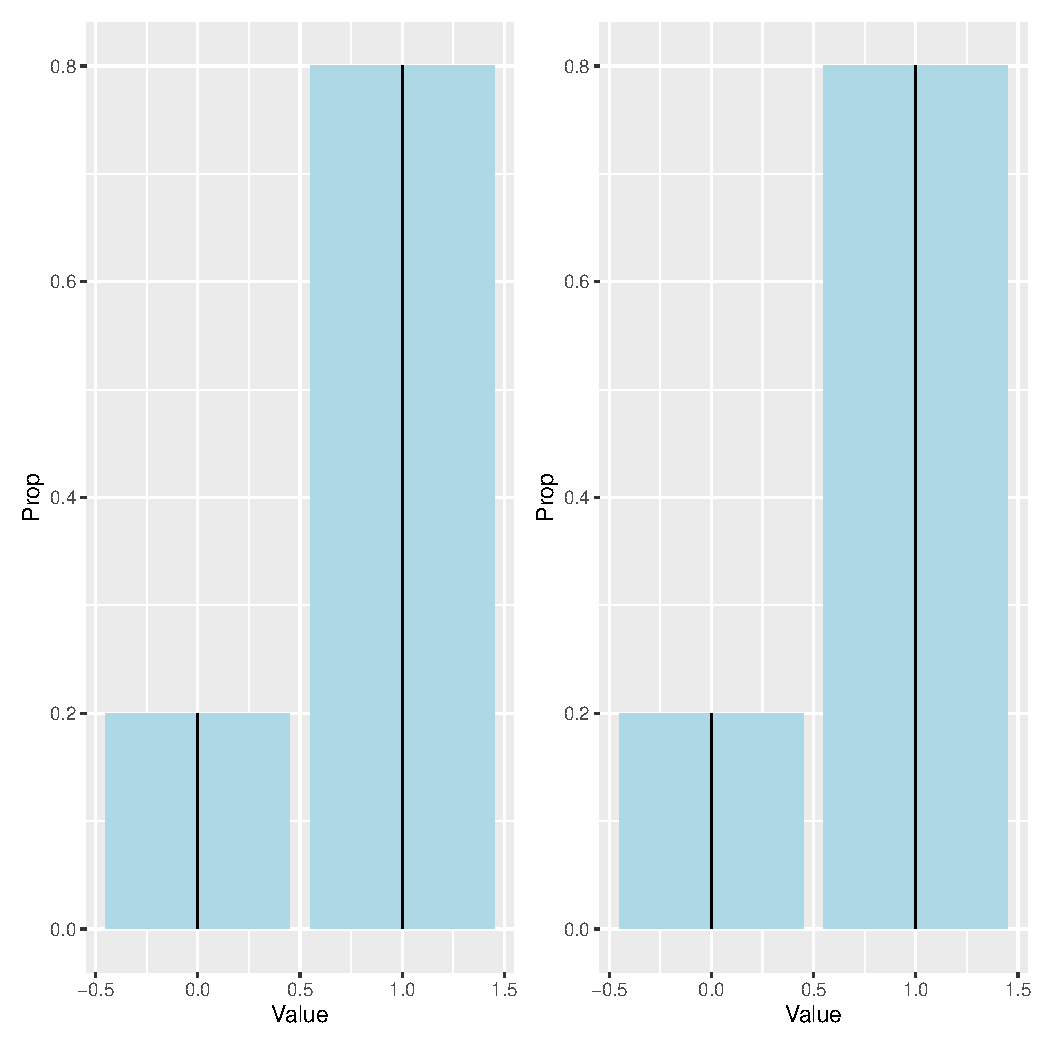
\includegraphics[width=\maxwidth]{figure/unnamed-chunk-4-1} 
\end{knitrout}
    \caption{Bernoulli($n=10$, $p=.5$)}
    \label{p4plot1}%we can now reference P3fig_1
  \end{center}
\end{figure}

\begin{knitrout}
\definecolor{shadecolor}{rgb}{0.969, 0.969, 0.969}\color{fgcolor}\begin{kframe}
\begin{alltt}
\hlstd{uneven.10} \hlkwb{<-} \hlkwd{rbinom}\hlstd{(}\hlkwc{n}\hlstd{=}\hlnum{10}\hlstd{,}        \hlcom{#number of observations}
                    \hlkwc{size}\hlstd{=}\hlnum{1}\hlstd{,}        \hlcom{#number of trials (size=1 for a Bernoulli distribution)}
                    \hlkwc{prob}\hlstd{=}\hlnum{.7}\hlstd{)}       \hlcom{#probability of success}

\hlkwd{paste}\hlstd{(}\hlstr{"MOM: "}\hlstd{,} \hlkwd{MOM.bernoulli}\hlstd{(uneven.10),}
      \hlstr{"MLE: "}\hlstd{,} \hlkwd{MLE.bernoulli}\hlstd{(uneven.10))}
\end{alltt}
\begin{verbatim}
## [1] "MOM:  0.8 MLE:  0.800000004445468"
\end{verbatim}
\end{kframe}
\end{knitrout}
Plot is Given Below:
\begin{knitrout}
\definecolor{shadecolor}{rgb}{0.969, 0.969, 0.969}\color{fgcolor}\begin{kframe}
\begin{alltt}
\hlkwd{bernoulli.plot}\hlstd{(uneven.10)}
\end{alltt}
\end{kframe}
\end{knitrout}
\begin{figure}[H]
  \begin{center}
  % This code is evaluated, but not printed
  % note below I use message=FALSE and warning=FALSE to surpress what's printed
  % when running library(ggmap) or library(patchwork) which would otherwise cause
  % an error because Sweave is expecting just a graph (not a graph + text)
\begin{knitrout}
\definecolor{shadecolor}{rgb}{0.969, 0.969, 0.969}\color{fgcolor}
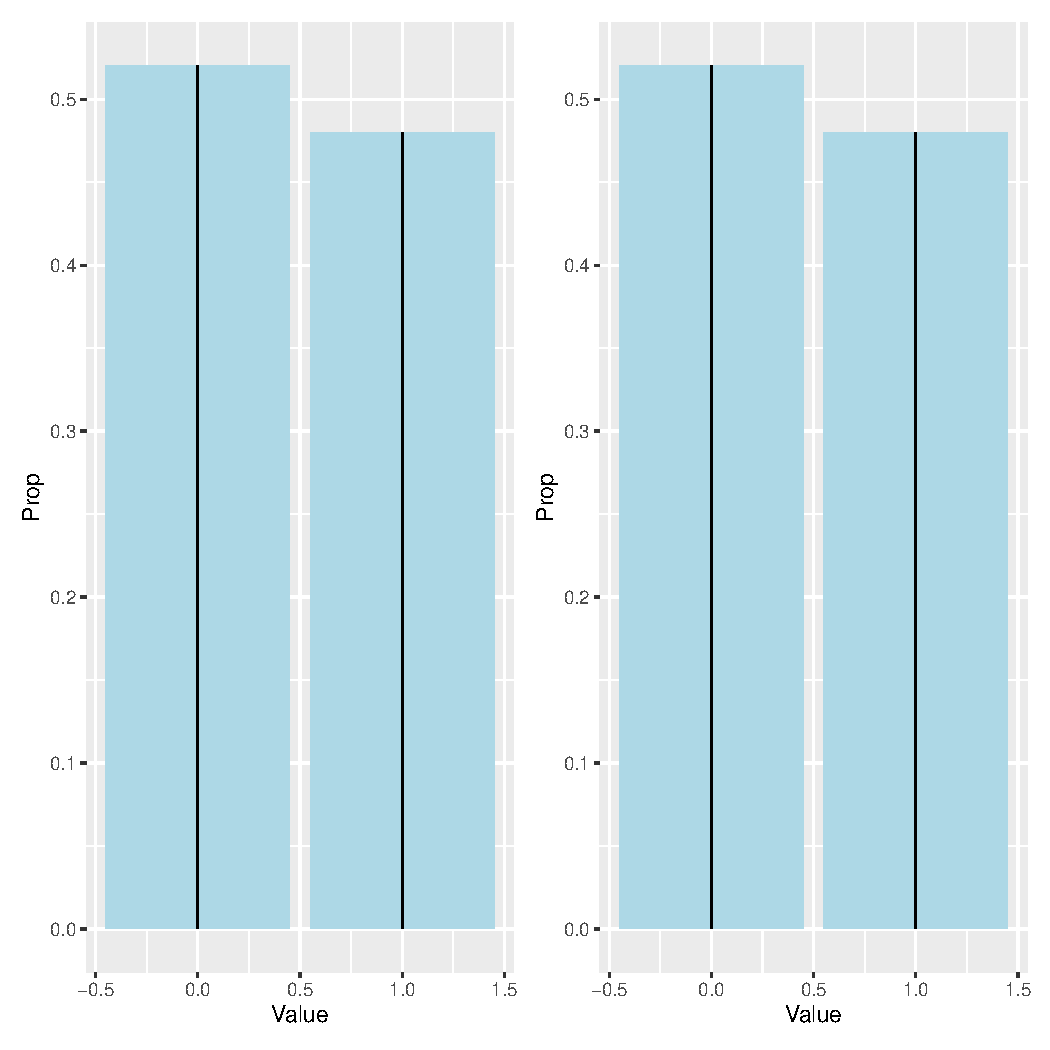
\includegraphics[width=\maxwidth]{figure/unnamed-chunk-6-1} 
\end{knitrout}
    \caption{caption here}
    \label{p4plot2}%we can now reference P3fig_1
  \end{center}
\end{figure}
  %%%%%%%%%%%%%%%%%%%%%%%%%%%%%%%%%%%%%%%%%%%%%%%%%%%%%%%%%%%%%%%%%%%%%%%%%%%%%%%%%%%%%%%%%%%
  %%%%%%%%%  Part (d)
  %%%%%%%%%%%%%%%%%%%%%%%%%%%%%%%%%%%%%%%%%%%%%%%%%%%%%%%%%%%%%%%%%%%%%%%%%%%%%%%%%%%%%%%%%%%
  \item Generate a random sample of size $n=25$ for your two sets of parameter(s). 
  Calculate the method of moments estimator(s) and maximum likelihood estimator(s).
  In a $1 \times 2$ grid, plot a histogram (with bin size 1) of each set of data 
  with (1) the method of moments estimated distribution, (2) the maximum likelihood 
  estimated distribution, and superimpose the true distribution in both.
\begin{knitrout}
\definecolor{shadecolor}{rgb}{0.969, 0.969, 0.969}\color{fgcolor}\begin{kframe}
\begin{alltt}
\hlstd{even.25} \hlkwb{<-} \hlkwd{rbinom}\hlstd{(}\hlkwc{n}\hlstd{=}\hlnum{25}\hlstd{,}        \hlcom{#number of observations}
                  \hlkwc{size}\hlstd{=}\hlnum{1}\hlstd{,}        \hlcom{#number of trials (size=1 for Bernoulli)}
                  \hlkwc{prob}\hlstd{=}\hlnum{.5}\hlstd{)}       \hlcom{#probability of success}

\hlkwd{paste}\hlstd{(}\hlstr{"MOM:"}\hlstd{,} \hlkwd{MOM.bernoulli}\hlstd{(even.25),}
      \hlstr{"MLE:"}\hlstd{,} \hlkwd{round}\hlstd{(}\hlkwd{MLE.bernoulli}\hlstd{(even.25),}\hlnum{2}\hlstd{))}
\end{alltt}
\begin{verbatim}
## [1] "MOM: 0.52 MLE: 0.52"
\end{verbatim}
\end{kframe}
\end{knitrout}
Plot is Given Below:
\begin{knitrout}
\definecolor{shadecolor}{rgb}{0.969, 0.969, 0.969}\color{fgcolor}\begin{kframe}
\begin{alltt}
\hlkwd{bernoulli.plot}\hlstd{(even.25)}
\end{alltt}
\end{kframe}
\end{knitrout}
\begin{figure}[H]
  \begin{center}
  % This code is evaluated, but not printed
  % note below I use message=FALSE and warning=FALSE to surpress what's printed
  % when running library(ggmap) or library(patchwork) which would otherwise cause
  % an error because Sweave is expecting just a graph (not a graph + text)
\begin{knitrout}
\definecolor{shadecolor}{rgb}{0.969, 0.969, 0.969}\color{fgcolor}
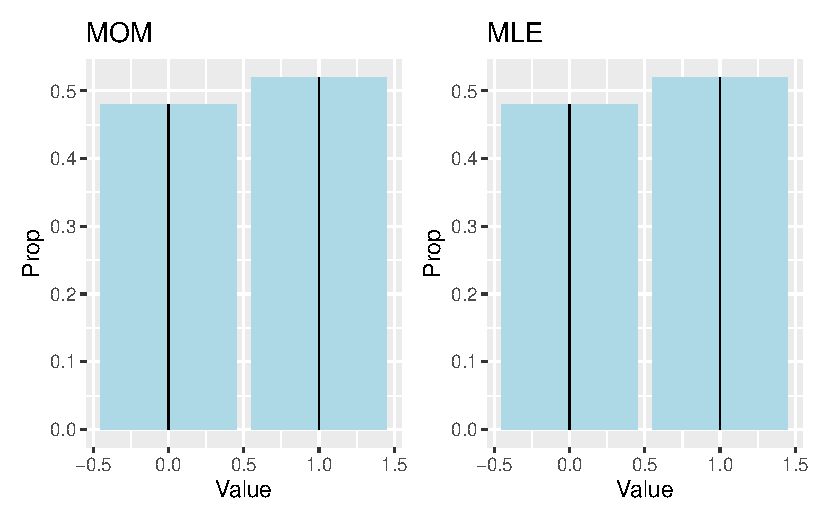
\includegraphics[width=\maxwidth]{figure/unnamed-chunk-8-1} 
\end{knitrout}
    \caption{caption here}
    \label{p4plot3}%we can now reference P3fig_1
  \end{center}
\end{figure}
\begin{knitrout}
\definecolor{shadecolor}{rgb}{0.969, 0.969, 0.969}\color{fgcolor}\begin{kframe}
\begin{alltt}
\hlstd{uneven.25} \hlkwb{<-} \hlkwd{rbinom}\hlstd{(}\hlkwc{n}\hlstd{=}\hlnum{25}\hlstd{,}        \hlcom{#number of observations}
                    \hlkwc{size}\hlstd{=}\hlnum{1}\hlstd{,}        \hlcom{#number of trials (size=1 for Bernoulli)}
                    \hlkwc{prob}\hlstd{=}\hlnum{.7}\hlstd{)}       \hlcom{#probability of success}

\hlkwd{paste}\hlstd{(}\hlstr{"MOM:"}\hlstd{,} \hlkwd{MOM.bernoulli}\hlstd{(uneven.25),}
      \hlstr{"MLE:"}\hlstd{,} \hlkwd{round}\hlstd{(}\hlkwd{MLE.bernoulli}\hlstd{(uneven.25),}\hlnum{2}\hlstd{))}
\end{alltt}
\begin{verbatim}
## [1] "MOM: 0.68 MLE: 0.68"
\end{verbatim}
\end{kframe}
\end{knitrout}
Plot is Given Below:
\begin{knitrout}
\definecolor{shadecolor}{rgb}{0.969, 0.969, 0.969}\color{fgcolor}\begin{kframe}
\begin{alltt}
\hlkwd{bernoulli.plot}\hlstd{(uneven.25)}
\end{alltt}
\end{kframe}
\end{knitrout}
\begin{figure}[H]
  \begin{center}
  % This code is evaluated, but not printed
  % note below I use message=FALSE and warning=FALSE to surpress what's printed
  % when running library(ggmap) or library(patchwork) which would otherwise cause
  % an error because Sweave is expecting just a graph (not a graph + text)
\begin{knitrout}
\definecolor{shadecolor}{rgb}{0.969, 0.969, 0.969}\color{fgcolor}
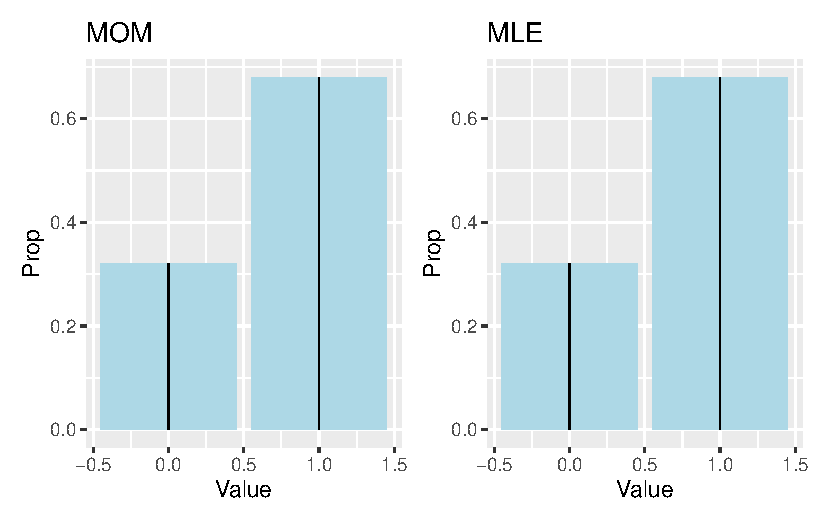
\includegraphics[width=\maxwidth]{figure/unnamed-chunk-10-1} 
\end{knitrout}
    \caption{caption here}
    \label{p4plot4}%we can now reference P3fig_1
  \end{center}
\end{figure}
  %%%%%%%%%%%%%%%%%%%%%%%%%%%%%%%%%%%%%%%%%%%%%%%%%%%%%%%%%%%%%%%%%%%%%%%%%%%%%%%%%%%%%%%%%%%
  %%%%%%%%%  Part (e)
  %%%%%%%%%%%%%%%%%%%%%%%%%%%%%%%%%%%%%%%%%%%%%%%%%%%%%%%%%%%%%%%%%%%%%%%%%%%%%%%%%%%%%%%%%%%
  \item Generate a random sample of size $n=100$ for your two sets of parameter(s).
  Calculate the method of moments estimator(s) and maximum likelihood estimator(s). 
  In a $1 \times 2$ grid, plot a histogram (with bin size 1) of each set of data 
  with (1) the method of moments estimated distribution, (2) the maximum likelihood
  estimated distribution, and superimpose the true distribution in both.
\begin{knitrout}
\definecolor{shadecolor}{rgb}{0.969, 0.969, 0.969}\color{fgcolor}\begin{kframe}
\begin{alltt}
\hlstd{even.100} \hlkwb{<-} \hlkwd{rbinom}\hlstd{(}\hlkwc{n}\hlstd{=}\hlnum{100}\hlstd{,}        \hlcom{#number of observations}
                  \hlkwc{size}\hlstd{=}\hlnum{1}\hlstd{,}        \hlcom{#number of trials (size=1 for Bernoulli)}
                  \hlkwc{prob}\hlstd{=}\hlnum{.5}\hlstd{)}       \hlcom{#probability of success}

\hlkwd{paste}\hlstd{(}\hlstr{"MOM:"}\hlstd{,} \hlkwd{round}\hlstd{(}\hlkwd{MOM.bernoulli}\hlstd{(even.100),}\hlnum{2}\hlstd{),}
      \hlstr{"MLE:"}\hlstd{,} \hlkwd{round}\hlstd{(}\hlkwd{MLE.bernoulli}\hlstd{(even.100),} \hlnum{2}\hlstd{))}
\end{alltt}
\begin{verbatim}
## [1] "MOM: 0.43 MLE: 0.43"
\end{verbatim}
\end{kframe}
\end{knitrout}
Plot is Given Below:
\begin{knitrout}
\definecolor{shadecolor}{rgb}{0.969, 0.969, 0.969}\color{fgcolor}\begin{kframe}
\begin{alltt}
\hlkwd{bernoulli.plot}\hlstd{(even.100)}
\end{alltt}
\end{kframe}
\end{knitrout}
\begin{figure}[H]
  \begin{center}
  % This code is evaluated, but not printed
  % note below I use message=FALSE and warning=FALSE to surpress what's printed
  % when running library(ggmap) or library(patchwork) which would otherwise cause
  % an error because Sweave is expecting just a graph (not a graph + text)
\begin{knitrout}
\definecolor{shadecolor}{rgb}{0.969, 0.969, 0.969}\color{fgcolor}
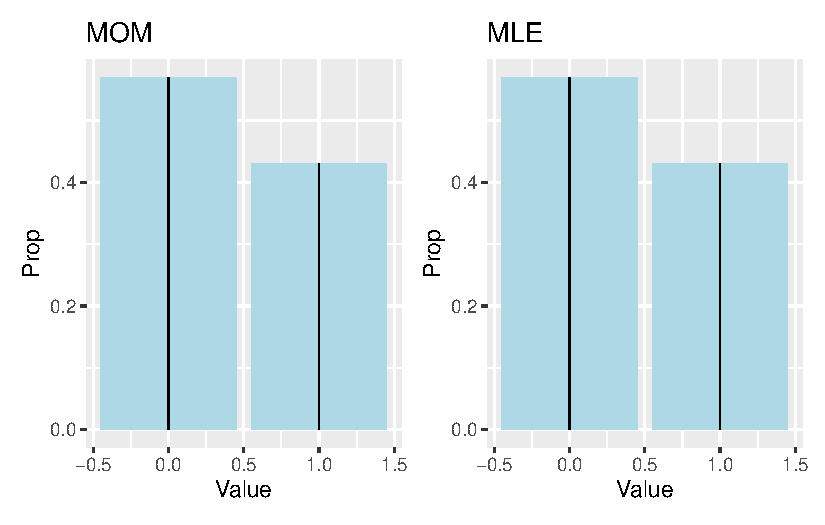
\includegraphics[width=\maxwidth]{figure/unnamed-chunk-12-1} 
\end{knitrout}
    \caption{caption here}
    \label{p4plot5}%we can now reference P3fig_1
  \end{center}
\end{figure}
\begin{knitrout}
\definecolor{shadecolor}{rgb}{0.969, 0.969, 0.969}\color{fgcolor}\begin{kframe}
\begin{alltt}
\hlstd{uneven.100} \hlkwb{<-} \hlkwd{rbinom}\hlstd{(}\hlkwc{n}\hlstd{=}\hlnum{100}\hlstd{,}        \hlcom{#number of observations}
                    \hlkwc{size}\hlstd{=}\hlnum{1}\hlstd{,}        \hlcom{#number of trials (size=1 for Bernoulli)}
                    \hlkwc{prob}\hlstd{=}\hlnum{.7}\hlstd{)}       \hlcom{#probability of success}

\hlkwd{paste}\hlstd{(}\hlstr{"MOM:"}\hlstd{,} \hlkwd{round}\hlstd{(}\hlkwd{MOM.bernoulli}\hlstd{(uneven.100),}\hlnum{2}\hlstd{),}
      \hlstr{"MLE:"}\hlstd{,} \hlkwd{round}\hlstd{(}\hlkwd{MLE.bernoulli}\hlstd{(uneven.100),} \hlnum{2}\hlstd{))}
\end{alltt}
\begin{verbatim}
## [1] "MOM: 0.81 MLE: 0.81"
\end{verbatim}
\end{kframe}
\end{knitrout}
Plot is Given Below:
\begin{knitrout}
\definecolor{shadecolor}{rgb}{0.969, 0.969, 0.969}\color{fgcolor}\begin{kframe}
\begin{alltt}
\hlkwd{bernoulli.plot}\hlstd{(uneven.100)}
\end{alltt}
\end{kframe}
\end{knitrout}
\begin{figure}[H]
  \begin{center}
  % This code is evaluated, but not printed
  % note below I use message=FALSE and warning=FALSE to surpress what's printed
  % when running library(ggmap) or library(patchwork) which would otherwise cause
  % an error because Sweave is expecting just a graph (not a graph + text)
\begin{knitrout}
\definecolor{shadecolor}{rgb}{0.969, 0.969, 0.969}\color{fgcolor}
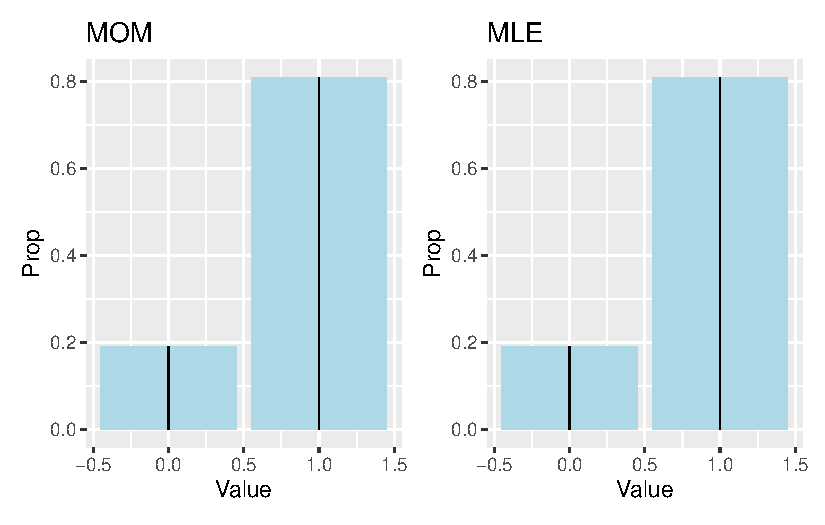
\includegraphics[width=\maxwidth]{figure/unnamed-chunk-14-1} 
\end{knitrout}
    \caption{caption here}
    \label{p4plot6}%we can now reference P3fig_1
  \end{center}
\end{figure}
  %%%%%%%%%%%%%%%%%%%%%%%%%%%%%%%%%%%%%%%%%%%%%%%%%%%%%%%%%%%%%%%%%%%%%%%%%%%%%%%%%%%%%%%%%%%
  %%%%%%%%%  Part (f)
  %%%%%%%%%%%%%%%%%%%%%%%%%%%%%%%%%%%%%%%%%%%%%%%%%%%%%%%%%%%%%%%%%%%%%%%%%%%%%%%%%%%%%%%%%%%
  \item Generate a random sample of size $n=100$ for your two sets of parameter(s).
  Calculate the method of moments estimator(s) and maximum likelihood estimator(s).
  In a $1 \times 2$ grid, plot a histogram (with bin size 1) of each set of data 
  with (1) the method of moments estimated distribution, (2) the maximum likelihood
  estimated distribution, and superimpose the true distribution in both.
\begin{knitrout}
\definecolor{shadecolor}{rgb}{0.969, 0.969, 0.969}\color{fgcolor}\begin{kframe}
\begin{alltt}
\hlstd{even.1000} \hlkwb{<-} \hlkwd{rbinom}\hlstd{(}\hlkwc{n}\hlstd{=}\hlnum{1000}\hlstd{,}        \hlcom{#number of observations}
                  \hlkwc{size}\hlstd{=}\hlnum{1}\hlstd{,}        \hlcom{#number of trials (size=1 for Bernoulli)}
                  \hlkwc{prob}\hlstd{=}\hlnum{.5}\hlstd{)}       \hlcom{#probability of success}

\hlkwd{paste}\hlstd{(}\hlstr{"MOM:"}\hlstd{,} \hlkwd{round}\hlstd{(}\hlkwd{MOM.bernoulli}\hlstd{(even.1000),}\hlnum{2}\hlstd{),}
      \hlstr{"MLE:"}\hlstd{,} \hlkwd{round}\hlstd{(}\hlkwd{MLE.bernoulli}\hlstd{(even.1000),} \hlnum{2}\hlstd{))}
\end{alltt}
\begin{verbatim}
## [1] "MOM: 0.5 MLE: 0.5"
\end{verbatim}
\end{kframe}
\end{knitrout}
Plot is given below:
\begin{knitrout}
\definecolor{shadecolor}{rgb}{0.969, 0.969, 0.969}\color{fgcolor}\begin{kframe}
\begin{alltt}
\hlkwd{bernoulli.plot}\hlstd{(even.1000)}
\end{alltt}
\end{kframe}
\end{knitrout}

\begin{figure}[H]
\begin{center}
\begin{knitrout}
\definecolor{shadecolor}{rgb}{0.969, 0.969, 0.969}\color{fgcolor}
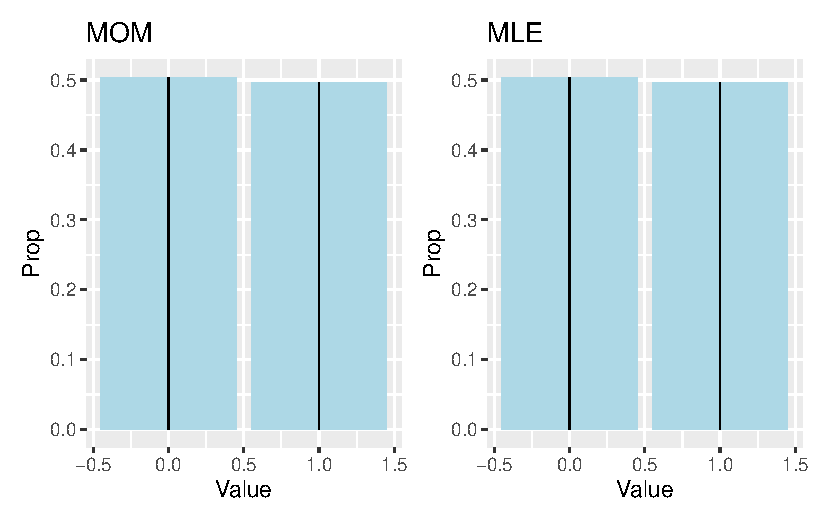
\includegraphics[width=\maxwidth]{figure/unnamed-chunk-16-1} 
\end{knitrout}
\caption{caption here}
\label{p4plot7}%we can now reference P3fig_1
\end{center}
\end{figure}


\begin{knitrout}
\definecolor{shadecolor}{rgb}{0.969, 0.969, 0.969}\color{fgcolor}\begin{kframe}
\begin{alltt}
\hlstd{uneven.1000} \hlkwb{<-} \hlkwd{rbinom}\hlstd{(}\hlkwc{n}\hlstd{=}\hlnum{1000}\hlstd{,}        \hlcom{#number of observations}
                    \hlkwc{size}\hlstd{=}\hlnum{1}\hlstd{,}        \hlcom{#number of trials (size=1 for Bernoulli)}
                    \hlkwc{prob}\hlstd{=}\hlnum{.7}\hlstd{)}       \hlcom{#probability of success}

\hlkwd{MOM.bernoulli}\hlstd{(uneven.1000)}
\end{alltt}
\begin{verbatim}
## [1] 0.734
\end{verbatim}
\begin{alltt}
\hlkwd{MLE.bernoulli}\hlstd{(uneven.1000)}
\end{alltt}
\begin{verbatim}
## [1] 0.734
\end{verbatim}
\begin{alltt}
\hlkwd{paste}\hlstd{(}\hlstr{"MOM:"}\hlstd{,} \hlkwd{round}\hlstd{(}\hlkwd{MOM.bernoulli}\hlstd{(uneven.1000),}\hlnum{2}\hlstd{),}
      \hlstr{"MLE:"}\hlstd{,} \hlkwd{round}\hlstd{(}\hlkwd{MLE.bernoulli}\hlstd{(uneven.1000),} \hlnum{2}\hlstd{))}
\end{alltt}
\begin{verbatim}
## [1] "MOM: 0.73 MLE: 0.73"
\end{verbatim}
\end{kframe}
\end{knitrout}
Plot is given below:
\begin{knitrout}
\definecolor{shadecolor}{rgb}{0.969, 0.969, 0.969}\color{fgcolor}\begin{kframe}
\begin{alltt}
\hlkwd{bernoulli.plot}\hlstd{(uneven.1000)}
\end{alltt}
\end{kframe}
\end{knitrout}

\begin{figure}[H]
\begin{center}
\begin{knitrout}
\definecolor{shadecolor}{rgb}{0.969, 0.969, 0.969}\color{fgcolor}
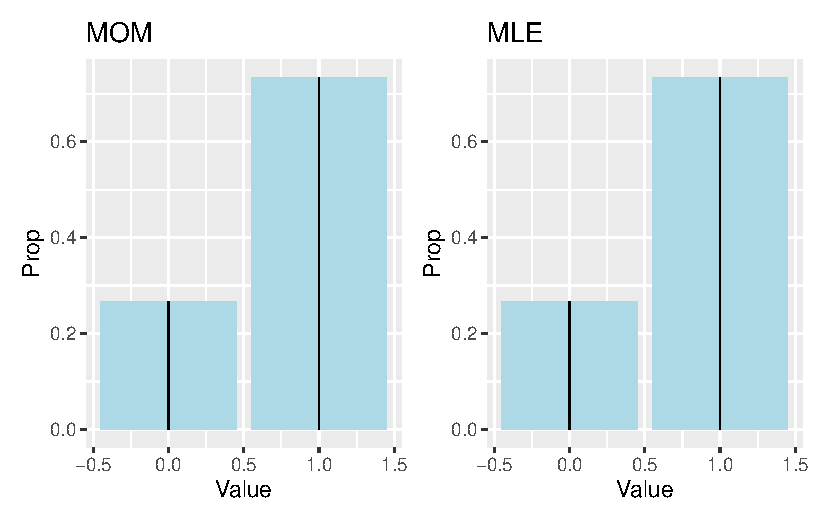
\includegraphics[width=\maxwidth]{figure/unnamed-chunk-18-1} 
\end{knitrout}
\caption{caption here}
\label{p4plot8}%we can now reference P3fig_1
\end{center}
\end{figure}
  %%%%%%%%%%%%%%%%%%%%%%%%%%%%%%%%%%%%%%%%%%%%%%%%%%%%%%%%%%%%%%%%%%%%%%%%%%%%%%%%%%%%%%%%%%%
  %%%%%%%%%  Part (g)
  %%%%%%%%%%%%%%%%%%%%%%%%%%%%%%%%%%%%%%%%%%%%%%%%%%%%%%%%%%%%%%%%%%%%%%%%%%%%%%%%%%%%%%%%%%%
  \item Comment on the results of parts (c)-(f). 
  \\
  \\
  From the plots in the results of parts (c)-(f), we can see that both the Method of Moments estimator and the Maximum Likelihood Estimator were able to provide a perfect estimate for the parameter $p$ regardless of our random sample size $n$. Therefore, I feel it is reasonable to conclude that using larger random sample sizes to find the MOM and MLE of a Bernoulli distribution is unnecessary.  \\
  \\
\end{enumerate}
\end{enumerate}%End overall enumerate
\newpage
\bibliography{bib}
\end{document}
